\begin{frame}{What is R Markdown?}

\begin{itemize}[<+->]
\itemsep1pt\parskip0pt\parsep0pt
\item
  source file / output file paradigm (cp LaTeX, HTML, markdown)
\item
  plain text file (.Rmd), rendered by R
\item
  markdown = plain-text authoring syntax, increasingly popular
  (e.g.~GitHub)
\item
  R Markdown = implementation of markdown, can take R code chunks
\item
  uses \texttt{knitr} package (successor to \texttt{Sweave}) and
  `Pandoc' text file conversion program
\item
  can produce HTML, PDF and Word documents
\item
  maintained by R Studio, now R Markdown v2
\end{itemize}

\end{frame}

\begin{frame}{What is R Markdown?}

\begin{itemize}[<+->]
\itemsep1pt\parskip0pt\parsep0pt
\item
  \textbf{simple syntax}: shallow learning curve
\item
  \textbf{human-readable}: emphasis on communication and clarity, rather
  than technique and complexity
\item
  \textbf{transparent formatting}: wysiwyg
\item
  \textbf{embedded computation}: share with collaborators, reviewers,
  colleagues, students, critics
\end{itemize}

\end{frame}

\begin{frame}{What is R Markdown?}

\begin{quote}
\ldots{} integrating source code, statistical output, and text in R
Markdown is \textbf{a model of reproducibility}.
\end{quote}

\begin{quote}
Such transparency facilitates comprehension, defensibility, and further
research or testing.
\end{quote}

\begin{quote}
R Markdown helps to bring the vision for reproducibility in statistical
analysis articulated by Gentleman \& Temple Lang {[}2004{]} to reality.
\end{quote}

\begin{itemize}[<+->]
\itemsep1pt\parskip0pt\parsep0pt
\item
  \href{http://onlinelibrary.wiley.com/doi/10.1002/wics.1348/abstract}{Baumer
  \& Udwin 2015, `R Markdown', \emph{WIRES: Computational Statistics}}
\end{itemize}

\end{frame}

\begin{frame}{How to use R Markdown}

\begin{block}{installation}

\begin{itemize}[<+->]
\itemsep1pt\parskip0pt\parsep0pt
\item
  \texttt{install.packages(\textquotesingle{}rmarkdown\textquotesingle{})}
\item
  \texttt{library(rmarkdown)}
\end{itemize}

\end{block}

\end{frame}

\begin{frame}{How to use R Markdown}

\begin{block}{simple syntax, human-readable, transparent formatting}

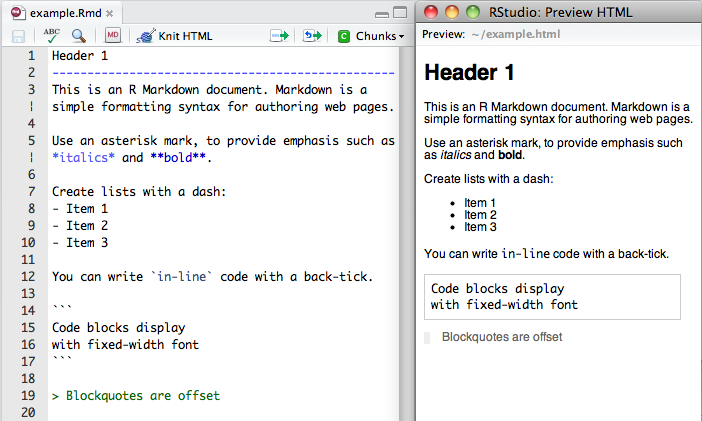
\includegraphics{images/markdownOverview.png}

\end{block}

\end{frame}

\begin{frame}{How to use R Markdown}

\begin{block}{embedded computation}

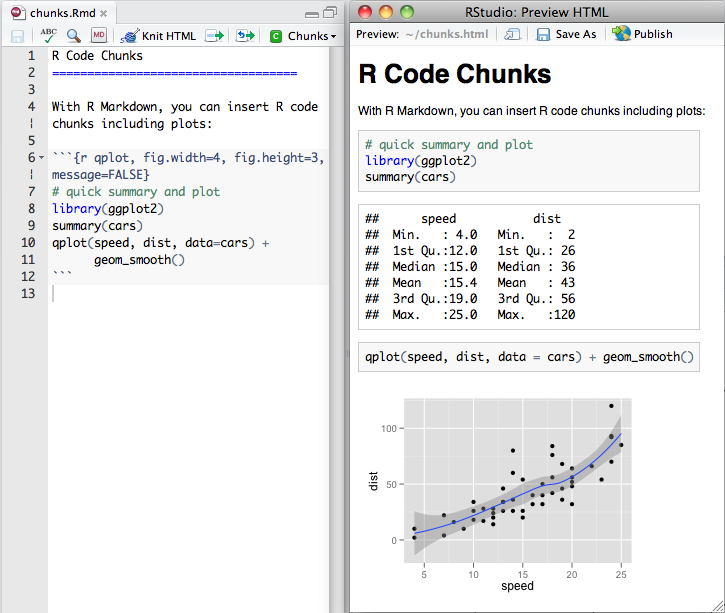
\includegraphics{images/markdownChunk.png}

\end{block}

\end{frame}

\begin{frame}{R Markdown and Reproducibility}

\begin{itemize}[<+->]
\itemsep1pt\parskip0pt\parsep0pt
\item
  User experience?
\item
  disappointing :-/
\item
  Computational linguistics \textgreater{}(open) Linguistics
\item
  culture of Shared Tasks, for example
\item
  Current project: proprietary data + 4p paper + no shared code +
  authors moved on
\item
  Martijn Wieling's statistics course:
  \href{http://www.let.rug.nl/~wieling/statscourse/lecture3/lab/answers/lab-including-answers.Rmd}{Rmd},
  \href{http://www.let.rug.nl/~wieling/statscourse/lecture3/lab/answers/lab-including-answers.html}{HTML}
\end{itemize}

\end{frame}

\begin{frame}{End}

\begin{block}{useful links}

\begin{itemize}
\itemsep1pt\parskip0pt\parsep0pt
\item
  \href{http://rmarkdown.rstudio.com/}{RStudio: R Markdown}
\item
  \href{http://arxiv.org/abs/1501.01613}{Udwin \& Baumer arXiv.org paper
  (= WIRES paper)}
\item
  \href{http://shiny.rstudio.com/articles/interactive-docs.html}{Shiny
  \& R Markdown}
\item
  \href{https://github.com/cainesap/replication}{my GitHub `replication'
  repo}
\end{itemize}

\end{block}

\begin{block}{contact me}

\begin{itemize}
\itemsep1pt\parskip0pt\parsep0pt
\item
  apc38
\item
  \href{http://apc38.user.srcf.net/}{my website}
\item
  {[}@cainesap{]}(\url{https://twitter.com/cainesap})
\end{itemize}

\end{block}

\end{frame}
